\documentclass[twoside,12pt]{article}
\usepackage[left=3.3cm,top=3.7cm,right=3.3cm,bottom=3.7cm,footskip=1.1cm]{geometry}

\newcommand{\omissis}{[\ldots\negthinspace]}

\renewcommand{\baselinestretch}{1}
\usepackage[utf8]{inputenc}
\usepackage{setspace}
\usepackage{amssymb}
\usepackage{ragged2e}
\usepackage{xcolor}
\usepackage{hyperref}
\hypersetup{
  colorlinks=true,
  linkcolor=blue!50!black,
  citecolor=blue!50!black}
  
\usepackage{geometry}
\usepackage{pifont}
\usepackage{amsmath}
\usepackage{lastpage}
\usepackage{adjustbox}
\usepackage{abstract}
\usepackage{anyfontsize}
\usepackage{breqn}
\usepackage{multirow}
\usepackage{caption}
\usepackage{graphicx}
\usepackage{subfig}
\usepackage{tabularx}
\usepackage{fancyhdr}
\usepackage{xcolor}
\usepackage{eurosym}
\usepackage{natbib}
%\bibliographystyle{agsm}
\bibliographystyle{aer}  % AER style
\usepackage{booktabs}

\makeatletter
\newenvironment{chapquote}[2][2em]
  {\setlength{\@tempdima}{#1}%
   \def\chapquote@author{#2}%
   \parshape 1 \@tempdima \dimexpr\textwidth-2\@tempdima\relax%
   \itshape}
  {\par \normalfont\hfill--\ \chapquote@author\hspace*{\@tempdima}\par\bigskip}
\makeatother

\pagestyle{fancy}
\fancyhf{}
\renewcommand{\headrulewidth}{0pt}
\fancyhead[RO,LE]{\large \thepage}
\fancyhead[CO]{\textit{\large Geographic Variation in Childhood Obesity}}
\fancyhead[CE]{\textit{\large Samuele Giambra}}
\fancyfoot[L,C,R]{}



\fancypagestyle{firststyle}
{
   \fancyhf{}
   \fancyfoot[C]{\large \thepage}
   \renewcommand{\headrulewidth}{0pt}
}
  
\newcommand{\yourname}{Samuele Giambra}
\newcommand{\youremail}{\url{giambar@hotmail.com}}

\hypersetup{urlcolor=blue!50!black}

%%%%%%%%%%%%%%%%%%%%%%%%%%%%%%%%%%%%%%%%%%
%here introduce cooler section titles  and abstract
\renewcommand{\thesection}{\Roman{section}} 
\renewcommand{\thesubsection}{\thesection.\Alph{subsection}}

\usepackage{titlesec}
\titleformat{\section}
  {\large\bfseries\centering}{\thesection.}{0.2em}{}
\titleformat{\subsection}
  {\normalfont\itshape\centering}{\thesubsection.}{0.3em}{}
 \titleformat{\subsubsection}
  {\normalfont\bfseries\itshape}{\thesubsubsection.}{0.3em}{}
  
\renewcommand{\abstractname}{}    % clear the title
\renewcommand{\absnamepos}{empty} % originally center
\usepackage{pdflscape}			  % rotates page
\usepackage{multirow}			  % introduces multiple rows in tables
\usepackage[capposition=top]{floatrow} 	% figure notes
\usepackage[space]{grffile}         	% figure path with spaces

  
%%%%%%%%%%%%%%%%%%%%%%%%%%%%%%%%%%%%%%%%%%%%%

\usepackage{epstopdf}		% needed for graphs
\usepackage{bm}				% for bold math symbols
\usepackage{tablefootnote}
\renewcommand*{\thefootnote}{\fnsymbol{footnote}}		% to use symbol in author pedices
\setcounter{footnote}{1}
\newcommand{\source}[1]{\caption*{\footnotesize{Source: {#1}}}} 	% add source to graphs
\usepackage[font={small}]{caption} 	% change font size captions
\usepackage[labelfont=bf]{caption}	% bold caption
\usepackage[shortlabels]{enumitem}	% allows to change bullet points into dash
\usepackage[flushleft]{threeparttable}	% includes notes in table environment
\usepackage{accents}
\newcommand\munderbar[1]{%
  \underaccent{\bar}{#1}}	%underbar in math mode

\newcommand*{\oneS}{\SuperScriptSameStyle{*}}
\newcommand*{\twoS}{\SuperScriptSameStyle{**}}
\newcommand*{\threeS}{\SuperScriptSameStyle{*{*}*}}
% commands for significance stars in tables

% double line in table
\newcommand\doubleRule{\toprule\toprule}
% specify path for figures
\graphicspath{{../../analysis/}}

\begin{document}\thispagestyle{firststyle}

\centerline{\Large{\textbf{Geographic Variation in Childhood Obesity:}}} 
\vspace{2mm}
\centerline{\large{\textbf{The effect of a healthier school environment}}} 

\vspace{5mm}

\centerline{\textit{By} SAMUELE GIAMBRA\footnote{Department of Economics, Brown University (e-mail: \href{mailto:samuele_giambra@brown.edu}{samuele\_giambra@brown.edu}).}} 


\vspace{8mm}
\renewcommand*{\thefootnote}{\arabic{footnote}}		% switch to numeric footnotes
\setcounter{footnote}{0}



%\onehalfspacing

\section{Introduction}
The obesity rate in the US has increased dramatically in the last decades. In the late 1970s, 12.7\% of men and 17\% of women were obese (cite). Today, almost one third of the population in the US could be classified as obese.\footnote{Between 2015 and 2016, 26.9\% of men and 27.6\% of women were obese (cite)} Despite the obesity rate is lower among younger Americans, childhood obesity remains a pervasive phenomenon. About 8.9\% of children between 2 and 5 years of age is currently obese. This percentage rises to 17.5\% for children of 6 to 11 years of age and 20.5\% for teenagers between 12 and 19 years old.  

This paper investigates whether school wellness policies are effective in addressing childhood obesity. 


On top of that, US obesity rate is characterized by a large geographic variation. \hyperref[cdc_obesity]{Figure 1} makes this point clear showing the percentage of obese population in 2013, by county.
\begin{figure}[htp]
  \centering
  \label{cdc_obesity}\caption{Percentage of obese population in 2013}
  \includegraphics[width=0.89\columnwidth]{C:/Users/giamb/Google Drive/research projects/obesity/maps/cdc_obesity_quintiles.png}
  \floatfoot{Notes: Data is from the Centers for Disease Control and Prevention (CDC) available at \url{https://www.cdc.gov/diabetes/atlas/countydata/atlas.html} as of December 2017. Counties are divided in five quantiles according to what fraction of the population is diagnosed as obese. Obesity rate in the US in 2013 ranged from 11.8\% to 47.6\%.}
\end{figure}
On average Southeastern states have a higher percentage of obese population than states on the West Coast. Income is clearly an important predictor for obesity, but uncovering which other factor drives geographic variation in obesity rates can have important policy implications. High obesity rates in the Southeast could be due to people intrinsic dietary preferences. \hyperref[adult_childhood_comparison]{Figure 1 A} in the appendix shows that there is a high degree of correlation between adult and childhood obesity rates.

A second related question is if students are affected by the health status of their peers.

 (see the right panel of \hyperref[windcapacity]{Figure 1}). 
\begin{figure}[h]\label{windcapacity}
\centering
\subfloat[BMI over lifetime]{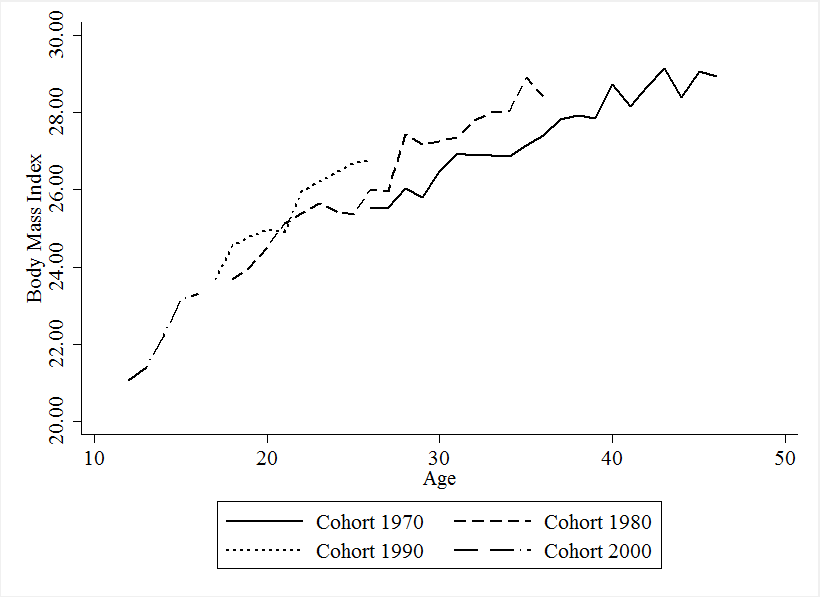
\includegraphics[width=70mm]{Cohort_plots_nhis/output/cohort_trend_bmi.png}}\hspace{1em}
\subfloat[US wind energy capacity]{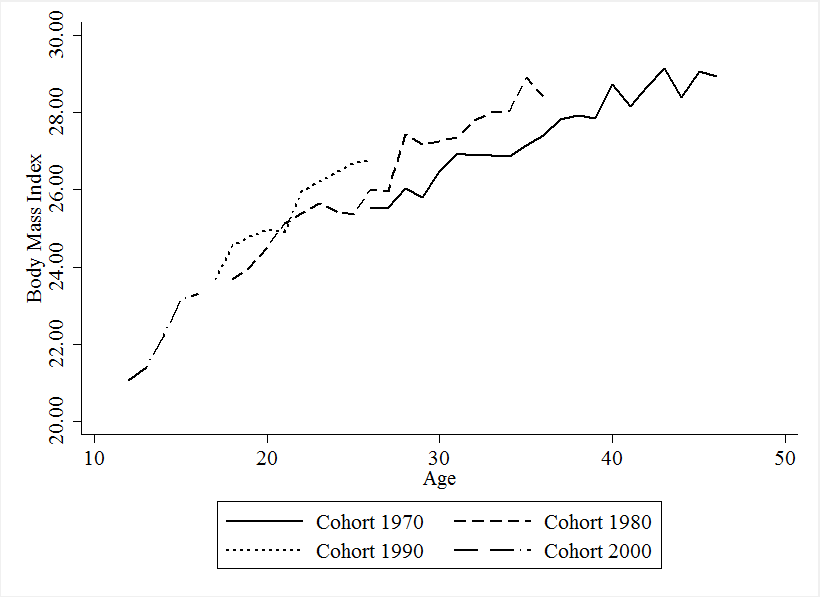
\includegraphics[width=70mm]{Cohort_plots_nhis/output/cohort_trend_bmi.png}}
\caption{Energy trends}
\end{figure}
Even if the public opinion is typically in favor of wind power \citep{firestone2007public}, the implementation of new wind turbine projects has often to overcome the opposition of local communities. A major concern is that the visual and aural impact of wind farms might decrease house values in the surrounding areas. For instance, \cite{slattery2012predominance} conduct surveys in several communities near wind farms in Texas and Iowa and find that one third of the respondents consider wind turbines an unattractive feature of the landscape. 

The object of this paper is to analyze the impact of the presence of wind turbines on house values. Using data on the location and building date of each turbine from the Federal Aviation Administration (FAA), and house prices collected from Zillow, I am able to estimate zip code level changes in house values for areas that are or are not allocated a wind turbine. However, the presence of a wind turbine in a given geographic area is clearly an endogenous outcome since infrastructure projects are usually targeted towards growing economic poles or influenced by political variables. I thus rely on two empirical strategies to try to isolate the causal impact of turbines on house prices. First, I instrument for wind turbines presence using the percentage of the area of each zip code where the average wind level is at least of category three. The underlying hypothesis is that higher wind power increases the benefits of building a wind turbine in that specific area. To do this, I match data on home selling prices per square foot with geographical and census data. Second, I perform an event study analysis to investigate how house values change in the years before and after a turbine is erected.

The results from the instrumental variable analysis show that wind turbines decrease the home selling price by slightly more than \$120 per square foot. This is a remarkable negative effect on house values considering that the mean of the distribution of median selling price per square foot in the US is about \$150. On the other hand, the results of the event study approach are more noisy and hence less informative about the impact of wind turbines on home prices. 

This paper mainly contributes to a recent literature that analyzes the detrimental effects of wind turbines on house transaction prices. \cite{sims2008modelling} are among the first to study this topic, using a sample of 201 house transactions within a mile of a wind farm in Cornwall, UK. The authors do not find any significant evidence of a causal effect of wind turbines on house prices, but this conclusion might be driven by the limitations of the data used. More recently, \cite{hoen2009impact} analyze the impact of 24 wind farms in the US using data on 7,500 sales of houses within 10 miles. In an improvement of this study, \cite{hoen2013spatial} use a difference-in-difference (DD) approach on more than 50,000 house transactions between 1996 and 2011 from areas within 10 miles of 67 wind farms in the US. Both of the aforementioned articles, however, are unable to uncover significant evidence of the impact of wind turbines on house prices. Focusing on Rhode Island, \cite{lang2014windy} use data from 3,254 transactions of houses within a mile of a wind turbine, finding no significant effect. A fair amount of other studies employing DD techniques have instead reached conclusions in favor of the hypothesis of a negative impact on house value. For the Netherlands, \cite{droes2014renewable} use 2.2 million transaction prices and find that the construction of a wind turbine lowers the price of houses within 2km by 1.4 percentage points. Similarly, \cite{sunak2016impact} find evidence of a negative impact of about 9-14\% in two German cities. \cite{gibbons2015gone} develop a slightly more articulated digital elevation model to create a 200m grid that shows if a turbine is visible or not from each location. The author uses then a DD comparing price changes in locations where a new turbine is built and is visible with different comparison groups, such as price changes in places where the new turbine is hidden by the terrain or became visible in the past. The main conclusion of the study is that visible wind turbines decrease house prices by 5-6\% within 2km, and by less than 1\% within 14km.

In this paper, I contribute to this literature in two different ways. First, I enlarge the scope of the analysis using data on wind turbines in each state of the US through September 2016. Second, in the preferred specification, I address the endogeneity issue of the allocation of a wind turbine to a given geographic area using an instrumental variable approach similar to the one exploited by \cite{dinkelman2011effects}, who instruments electrification projects in South Africa using land gradient. To my knowledge, this is the first attempt to use an IV approach to estimate the impact of wind turbines on house prices.

\section{Background}
To analyze how the presence of wind turbines affects house values, I construct a panel that covers the period from 2000 to 2016, where variables are aggregated at the zip code level. Median home selling prices per square foot are collected from Zillow\footnote{Zillow datasets are publicly available for download from the \href{http://www.zillow.com/research/data/}{data section on Zillow webpage}.}. All types of homes are considered, that is, all single-family, condominium and co-operative homes with a county record. Zillow provides other measures of home values, as for instance the Zillow Home Value Index (ZHVI) that measures the median seasonally adjusted home value for a given area. However, these metrics are the output of statistical models that take already into account characteristics such as local amenities and are thus less indicated for the current analysis. To the house prices panel I add data on wind turbines made available by the Federal Aviation Administration (FAA), which contains monthly data through September 2016 on the exact position of each wind turbine in the US\footnote{The actual GIS files are publicly available for download from the \href{https://www.fws.gov/southwest/es/Energy_Wind_FAA.html}{US Fish \& Wildlife Service website}.}. Records include undergoing projects, denied permissions, and locations under revision during the permission application process. 
\begin{figure}[htp]
  \centering
  \label{homestrend}\caption{Secular trend in teen BMI}
  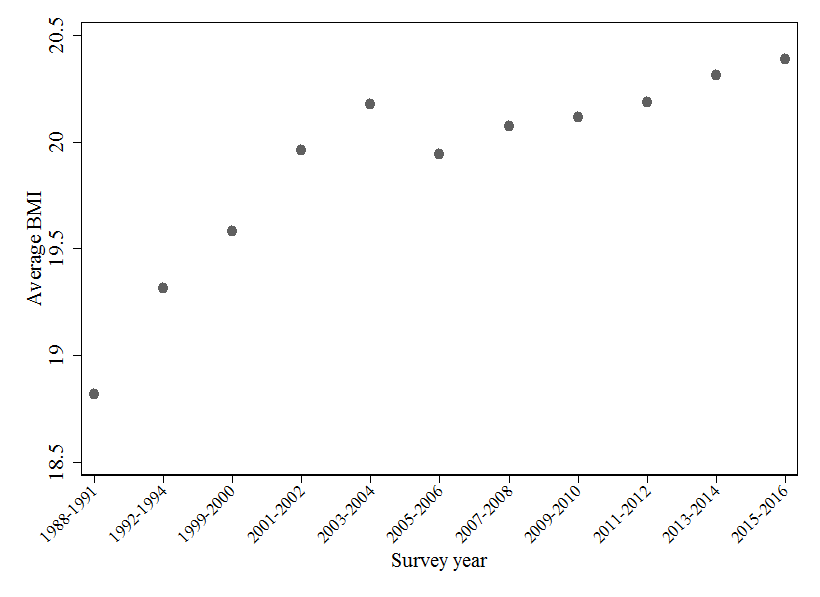
\includegraphics[width=100mm]{Trends_in_obesity_nhanes/output/bmi_2to18_nhanes.png}
  \floatfoot{Notes: Data is from the National Health and Nutrition Examination Survey (NHANES) III and 1999-2016 available at ... as of December 2017.}
\end{figure}

\section{Identification strategy}
If 

If the presence of a wind turbine in a given zip code was determined randomly, I could in principle be able to estimate its effect on house values using the following model
\begin{equation}\label{estimation}
y_{zst}=\alpha_0 + \alpha_1 t + \alpha_2 T_{zst} + \mu_z + \delta_z t + \rho_s + \lambda_s t + \epsilon_{zst},
\end{equation}
where $y_{zst}$ measures the average house value in zip code $z$, state $s$ and time $t$, and $T_{zst}$ captures whether a wind turbine is active in that location. The other parameters in the model -- $\mu_z$, $\delta_z$, $\rho_s$, and $\lambda_s$ -- capture fixed effects and trends for each zip code and state, respectively, while $\alpha_1$ measures time fixed effects. However, the coefficients estimated running simple OLS on \hyperref[estimation]{equation 1} are likely to be biased by the existence of omitted variables that are correlated with both the change in house values and wind turbine presence. For instance, if poorer geographic areas are more likely to be allocated a wind turbine, and the price of houses in these areas is lower, then this would generate a negative relationship between turbines and house prices. In the attempt to reduce this problem, I control for a vector of zip code level covariates,  $\mathbf{X}_{zs0}$, measured in 2000, the baseline period of the analysis. Among the control variables I include distance from the coastline; elevation; percentage of urbanized area; total population; fraction of whites, blacks and asians; income per capita; and educational attainment. Unfortunately, even after controlling for these zip code characteristics it is still likely that the estimate of $\alpha_2$ will be biased due to omitted or unobservable variables and confounding trends. To identify the causal impact of wind turbines on house values I therefore rely on an instrumental variable approach. I use annual average 50-meter height above the ground wind data to construct a variable that measures the percentage of the area of a given zip code having wind of power category equal or higher than three. Since the productivity of wind turbines depends, among other geographic characteristics, on the location's wind power, this instrument is likely to be a good predictor for wind turbine presence. The two equations related to the IV approach are the following
\begin{equation}\label{firststage}
\text{First stage: }\quad T_{zst}=\pi_0 + \pi_1 t + \pi_2 Z_{zt} + \mathbf{X}_{zs0} \boldsymbol{\pi}_{\mathbf{2}} + \gamma_s + \tau_{zst},
\end{equation}
\begin{equation}\label{secondstage}
\text{Second stage: }\quad y_{zst}=\alpha_0 + \alpha_1 t + \alpha_2 T_{zst} + \mathbf{X}_{zs0} \boldsymbol{\beta} +  \lambda_d + \epsilon_{zst}.
\end{equation}
\subsection{Movers}
\begin{figure}[htp]
  \centering
  \label{homestrend}\caption{Movers}
  \includegraphics[width=100mm]{C:/Users/giamb/Google Drive/research projects/obesity/maps/childhood_obesity_ny.PNG}
  \floatfoot{Notes: Data is from the New York State Department of Health available at ... as of December 2017.}
\end{figure}

\begin{figure}[htp]
  \centering
  \label{homestrend}\caption{Movers}
  \includegraphics[width=100mm]{C:/Users/giamb/Google Drive/research projects/obesity/maps/bmi_screening_states.PNG}
  \floatfoot{Notes: Table from \cite{linchey2011peer}.}
\end{figure}

\subsection{School eating environment}
\begin{figure}[htp]
  \centering
  \label{homestrend}\caption{CLASS 2003}
  \includegraphics[width=100mm]{C:/Users/giamb/Google Drive/research projects/obesity/maps/alacarte_beverages_2003.PNG}
  \floatfoot{Notes: Data is from the }
\end{figure}

\begin{figure}[htp]
  \centering
  \label{homestrend}\caption{CLASS 2015}
  \includegraphics[width=100mm]{C:/Users/giamb/Google Drive/research projects/obesity/maps/alacarte_beverages_2015.PNG}
  \floatfoot{Notes: Data is from the }
\end{figure}

\section{Planned estimation}


\newpage
\bibliography{Report}

\newpage
\section*{Appendix: Additional Figures and Tables}
\renewcommand{\thetable}{A.\arabic{table}}
\setcounter{table}{0}
\renewcommand{\thefigure}{A.\arabic{figure}}
\setcounter{figure}{0}
\renewcommand{\theequation}{A.\arabic{equation}}
\setcounter{equation}{0}
\renewcommand{\thesubsection}{A.\arabic{subsection}}
\setcounter{subsection}{0}

\begin{figure}[h]\label{adult_childhood_comparison}
	\centering
	\subfloat[Panel A]{%
  		\includegraphics[clip,width=0.89\columnwidth]{C:/Users/giamb/Google Drive/research projects/obesity/maps/cdc_adult_obesity.png}%
	} \\
	\subfloat[Panel B]{%
 		\includegraphics[clip,width=0.6\columnwidth]{C:/Users/giamb/Google Drive/research projects/obesity/maps/nhanes_childhood_obesity.png}%
	}
	\caption{Comparison between adult and childhood obesity rates, by county}
	\floatfoot{Notes: Panel A shows data on adult obesity from the Centers for Disease Control and Prevention (CDC) available at \url{https://www.cdc.gov/diabetes/atlas/countydata/atlas.html} as of December 2017. Panel B displays data on childhood obesity for all children age 5-17 from Childhood Obesity Index available at \url{http://maps.z-atlas.com/ChildhoodObesityIndex/main.cfm} as of December 2017. Darker-shaded counties have a higher adult/childhood obesity rate in 2008.}
\end{figure}


\end{document}